\section{Exploration and Analysis}
    % Suggested 500 words for individual report; proportionately longer for group
    % projects).

    % 't' means "try to position at the top of the page"
    \begin{figure}[t]
        \centering
        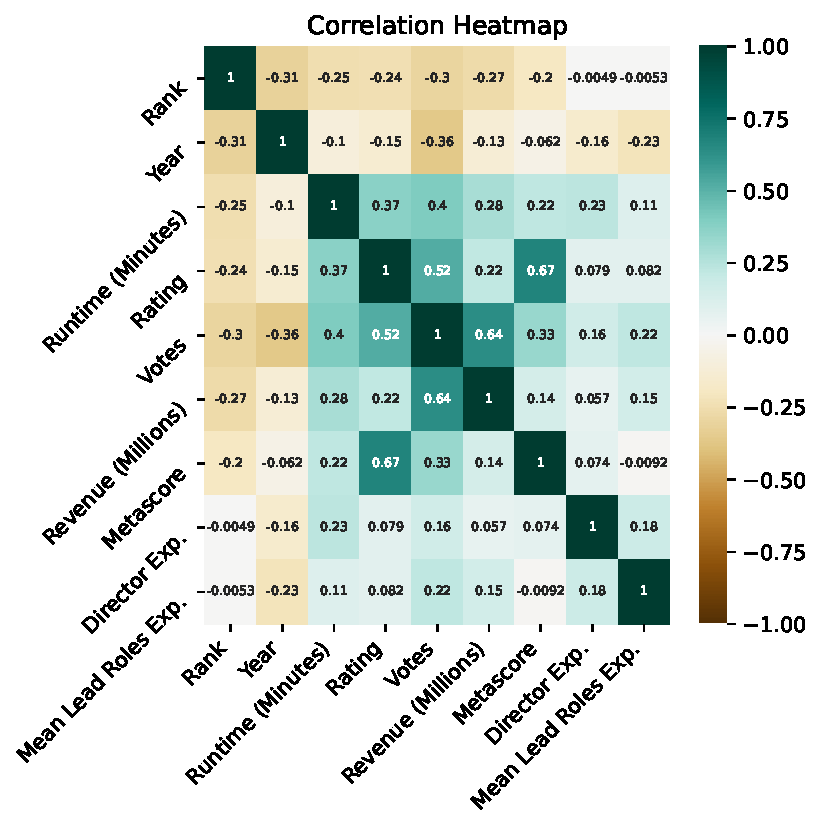
\includegraphics[scale=0.75]{Prelim Analysis/Correlation Heatmap.pdf}
        \caption{Demonstration figure.
            This caption explains more about the figure.
            Note that the font size of the labels in the plot is 9pt, which is obtained by
                the settings as shown in the Jupyter notebook.
        }
        \label{fds-project-template:fig:example1}
    \end{figure}

    % 'b' means "try to position at the bottom of the page"
    \begin{table}[b]
        \centering
        \caption{Excerpt from Scottish Index of Multiple Deprivation, 2016 edition.
            \url{https://simd.scot}.
            You may put more information in the caption.
        }
        \label{tab:example1}
        \begin{tabular}{lrrrrrrr}
            \hline\hline
            \textbf{Location} & \textbf{Employ-} & \textbf{Illness} & \textbf{Attain-} & \textbf{Drive}   & \textbf{Drive}     & \textbf{Crime} & \dots                \\
                              & \textbf{ment}    &                  & \textbf{ment}    & \textbf{Primary} & \textbf{Secondary} &                &                      \\
            \hline
            \textbf{Macduff}  & $10$             & $ 95$            & $5.3$            & $1.5$            & $6.6$              & $249$          & \dots\tabularnewline
            \textbf{Kemnay}   & $ 3$             & $ 40$            & $5.3$            & $2.4$            & $2.4$              & $168$          & \dots\tabularnewline
            \textbf{Hilton}   & $ 0$             & $ 10$            & $6.3$            & $2.2$            & $3.0$              & $144$          & \dots\tabularnewline
            \textbf{Ruchill}  & $ 8$             & $130$            & $4.9$            & $1.7$            & $5.6$              & $318$          & \dots\tabularnewline
            \textbf{Belmont}  & $ 2$             & $ 50$            & $6.1$            & $3.1$            & $3.2$              & $129$          & \dots\tabularnewline
            \dots             & \dots            & \dots            & \dots            & \dots            & \dots              & \dots          & \dots\tabularnewline
            \hline
        \end{tabular}
    \end{table}

    A data science analysis of the paper, including: \begin{itemize} \item
        Visualisations (for example Figure~\ref{fds-project-template:fig:example1}) and
        tables (for example Table~\ref{tab:example1}).
    Please make sure that all figures and tables are referred to in the text, as
        demonstrated in this bullet point.
    \item Interpretation of the results
    \item Description of how you have applied one ore more of the
    statistical and ML methods learned in the FDS to the data
    \item Interpretation of the findings
    \end{itemize}

    You can use equations like this:
    \begin{equation}
        \label{fds-project-template:eq:1} \overline{x} = \sum_{i=1}^n x_i
    \end{equation}
    or maths inline: $E=mc^2$.
    However, you do not need to reexplain techniques that you have learned in the
        course -- assume the reader understands linear regression, logistic regression
        K-nearest neighbours etc. Remember to explain any symbols use, e.g.~``$n$ is
        the number of data points and $x_i$ is the value of the $i$th data point.
    ''.